\begin{figure}[ht]
    \begin{center}
        \begin{minipage}[b]{0.48\textwidth}
            \centering
            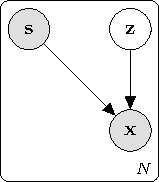
\includegraphics[scale=0.75]{unsupervised.pdf}
            \caption{Unsupervised model}
        \end{minipage}
        \quad
          \begin{minipage}[b]{0.48\textwidth}
            \centering
            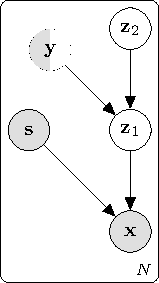
\includegraphics[scale=0.75]{semisupervised.pdf}
            \caption{Semi-supervised model}
        \end{minipage}
    \end{center}
\end{figure}

\subsection{Unsupervised model}
Factoring out undesired variations from the data can be easily formulated as a general probabilistic model which admits two distinct (independent) ``sources''; an observed variable $\*s$, which denotes the variations that we want to remove, and a continuous latent variable $\*z$ which models all the remaining information.  This generative process can be formally defined as:
\begin{align*}
	\*z \sim p(\*z); \qquad \*x \sim p_\theta(\*x| \*z, \*s)
\end{align*}
where $p_\theta(\*x| \*z, \*s)$ is an appropriate probability distribution for the data we are modelling. With this formulation we explicitly encode a notion of `invariance' in our model, since the latent representation is marginally independent of the factors of variation $\*s$. Therefore the problem of finding an invariant representation for a data point $\*x$ and variation $\*s$ can be cast as performing inference on this graphical model and obtaining the posterior distribution of $\*z$, $p(\*z|\*x, \*s)$. 

For our model we will employ a variational autoencoder architecture~\citep{kingma2013auto,rezende2014stochastic}; namely we will parametrize the generative model (decoder) $p_\theta(\*x|\*z,\*s)$ and  the variational posterior (encoder) $q_\phi(\*z|\*x,\*s)$ as (deep) neural networks which accept as inputs $\*z,\*s$ and $\*x,\*s$ respectively and produce the parameters of each distribution after a series of non-linear transformations. Both the model ($\theta$) and variational ($\phi$) parameters will be jointly optimized with the SGVB~\citep{kingma2013auto} algorithm according to a lower bound on the log-likelihood. This parametrization will allow us to capture most of the salient information of $\*x$ in our embedding $\*z$. Furthermore the distributed representation of a neural network would allow us to better resolve the dependencies between $\*x$ and $\*s$ thus yielding a better disentangling between the independent factors $\*z$ and $\*s$. By choosing a Gaussian posterior $q_\phi(\*z|\*x, \*s)$ and standard isotropic Gaussian prior $p(\*z) = \mathcal{N}(\*0, \*I)$ we can obtain the following lower bound:
\begin{align}
	\sum_{n=1}^{N}\log p(\*x_n|\*s_n) & \ge  \sum_{n=1}^{N}\E_{q_\phi(\*z_n|\*x_n,\*s_n)}[\log p_\theta(\*x_n|\*z_n,\*s_n)] - KL(q_\phi(\*z_n|\*x_n,\*s_n) || p(\*z))\\
	                    & = \mathcal{F}(\phi, \theta; \*x_n, \*s_n) \nonumber
\end{align}
with $q_\phi(\*z_n|\*x_n, \*s_n) = \mathcal{N}(\*z_n|\!\mu_n = f_\phi(\*x_n, \*s_n), \!\sigma_n = e^{f_\phi(\*x_n, \*s_n)})$ and $p_\theta(\*x_n|\*z_n, \*s_n) = f_\theta(\*z_n, \*s_n)$ with $f_\theta(\*z_n, \*s_n)$ being an appropriate probability distribution for the data we are modelling.

\subsection{Semi-Supervised model}
Factoring out variations in an unsupervised way can however be harmful in cases where we want to use this invariant representation for a subsequent prediction task. In particular if we have a situation where the nuisance variable $\*s$ and the actual label $\*y$ are correlated, then training an unsupervised model could yield \emph{random} or \emph{degenerate} representations with respect to $\*y$. Therefore it is more appropriate to try to ``inject'' the information about the label during the feature extraction phase. This can be quite simply achieved by introducing a second ``layer'' of latent variables to our generative model where we try to correlate $\*z$ with the prediction task. Assuming that the invariant features are now called $\*z_1$ we enrich the generative story by similarly providing two distinct (independent) sources for $\*z_1$; a discrete (in case of classification)variable $\*y$ which denotes the label of the data point $\*x$ and a continuous latent variable $\*z_2$ which encodes the variation on $\*z_1$ that is not explained by $\*y$ ($\*x$ dependent noise). The process now can be formally defined as: 
\begin{align*}
\*y, \*z_2 \sim \text{Cat}(\*y)p(\*z_2); \qquad  \*z_1 \sim p_\theta(\*z_1|\*z_2, \*y);\qquad \*x \sim p_\theta(\*x| \*z_1,\*s)\nonumber
\end{align*}   
Similarly to the unsupervised case we use a variational auto-encoder and jointly optimize the variational and model parameters. The lower bound now becomes:
\begin{align}
\sum_{n=1}^{N}\log p(\*x_n|\*s_n) & \ge \sum_{n=1}^{N}\E_{q_\phi({\*z_1}_n, {\*z_2}_n, \*y_n| \*x_n, \*s_n)}[\log p(\*z_2) + \log p(\*y_n) + \log p_\theta({\*z_1}_n|{\*z_2}_n, \*y_n) + \nonumber\\&\qquad\qquad\qquad\qquad + \log p_\theta(\*x_n|{\*z_1}_n,\*s_n) - \log q_\phi({\*z_1}_n, {\*z_2}_n, \*y_n|\*x_n, \*s_n)]  
\end{align}
where we assume that the posterior $q_\phi({\*z_1}_n, {\*z_2}_n, \*y_n|\*x_n, \*s_n)$ is factorized as $q_\phi({\*z_1}_n, {\*z_2}_n, \*y_n|\*x_n, \*s_n) = q_\phi({\*z_1}_n|\*x_n, \*s_n)q_\phi(\*y_n|{\*z_1}_n)q_\phi({\*z_2}_n|{\*z_1}_n,\*y_n)$, and where:
\begin{align*}
q_\phi({\*z_1}_n|\*x_n, \*s_n) & = \mathcal{N}({\*z_1}_n|\!\mu_n = f_\phi(\*x_n, \*s_n), \!\sigma_n = e^{f_\phi(\*x_n, \*s_n)}) \\
q_\phi(\*y_n | {\*z_1}_n) & = \text{Cat}(\*y_n|\!\pi_n = \text{softmax}(f_\phi({\*z_1}_n)))\\
q_\phi({\*z_2}_n|{\*z_1}_n, \*y_n) & = \mathcal{N}({\*z_2}_n| \!\mu_n = f_\phi({\*z_1}_n, \*y_n), \!\sigma_n = e^{f_\phi({\*z_1}_n, \*y_n)})\\
p_\theta({\*z_1}_n | {\*z_2}_n, \*y_n) & = \mathcal{N}({\*z_1}_n| \!\mu_n = f_\theta({\*z_2}_n, \*y_n), \!\sigma_n = e^{f_\theta({\*z_2}_n, \*y_n)})\\
p_\theta(\*x_n|{\*z_1}_n, \*s_n) & = f_\theta({\*z_1}_n, \*s_n)
\end{align*}
with $f_\theta({\*z_1}_n, \*s_n)$ again being an appropriate probability distribution for the data we are modelling. The model proposed here can be seen as an extension to the `stacked M1+M2' model originally proposed from~\cite{kingma2014semi}, where we have additionally introduced the nuisance variable $\*s$ during the feature extraction. Thus following~\cite{kingma2014semi} we can also handle the `semi-supervised' case, i.e., missing labels. In situations where the label is observed the lower bound takes the following form (exploiting the fact that we can compute some Kullback-Leibler divergences explicitly in our case):
\begin{align}
\sum_{n=1}^{N}\mathcal{L}_s(\phi, \theta; \*x_n, \*s_n, \*y_n) & =\sum_{n=1}^{N_s} \E_{q_\phi({\*z_1}_n|\*x_n, \*s_n)}[-KL(q_\phi({\*z_2}_n|{\*z_1}_n, \*y_n) || p(\*z_2)) + \log p_\theta(\*x_n|{\*z_1}_n, \*s_n)] +\nonumber\\&\qquad\qquad + \E_{q_\phi({\*z_1}_n|\*x_n, \*s_n)q_\phi({\*z_2}_n|{\*z_1}_n,\*y_n)}[\log p_\theta({\*z_1}|{\*z_2}_n, \*y_n)- \log q_\phi({\*z_1}_n|\*x_n \*s_n)]
\end{align}
and in the case that it is not observed we use $q(\*y_n|{\*z_1}_n)$ to `impute' our data:
\begin{align}
\sum_{m=1}^{M}\mathcal{L}_u(\phi, \theta; \*x_m, \*s_m) & = \sum_{m=1}^{M}\E_{q_\phi({\*z_1}_m|\*x_m,\*s_m)}[ - KL (q(\*y_m|{\*z_1}_m) || p(\*y_m)) + \log p_\theta(\*x_m|{\*z_1}_m, \*s_m)] +\nonumber\\&\qquad\qquad +  \E_{q_\phi({\*z_1}_m, \*y_m|\*x_m,\*s_m)}[ - KL (q_\phi({\*z_2}_m|{\*z_1}_m,\*y_m) || p(\*z_2))] +\nonumber\\&\qquad\qquad+  \E_{q_\phi({\*z_1}_m, \*y_m, {\*z_2}_m|\*x_m, \*s_m)}[\log p_\theta({\*z_1}_m|{\*z_2}_m,\*y_m) -\log q_\phi({\*z_1}_m|\*x_m,\*s_m) ]
\end{align}
therefore the final objective function is:
\begin{align}
    \mathcal{F}_{\text{VAE}}(\phi, \theta; \*x_n, \*x_m, \*s_n, \*s_m, \*y_n) & = \sum_{n=1}^{N}\mathcal{L}_s(\phi, \theta; \*x_n, \*s_n, \*y_n) + \sum_{m=1}^{M}\mathcal{L}_u(\phi, \theta; \*x_m, \*s_m) + \nonumber \\ &\qquad\qquad +  \alpha\sum_{n=1}^{N}\E_{q({\*z_1}_n|\*x_n, \*s_n)}[- \log q_\phi(\*y_n|{\*z_1}_n)]
\end{align}
where the last term is introduced so as to ensure that the predictive posterior $q_\phi(\*y|\*z_1)$ learns from both labeled and unlabeled data. This semi-supervised model will be called ``VAE'' in our experiments.

However, there is a subtle difference between the approach of~\cite{kingma2014semi} and our model. Instead of training separately each layer of stochastic variables we optimize the model jointly. The potential advantages of this approach are two fold: as we previously mentioned if the label $\*y$ and the nuisance information $\*s$ are correlated then training a (conditional) feature extractor separately poses the danger of creating a degenerate representation with respect to the label $\*y$. Furthermore the label information will also better guide the feature extraction towards the more salient parts of the data, thus maintaining most of the (predictive) information.
